\begin{figure}[t]
\centering
% Vector drawing generated by tools/figures/metric_record.py from the 10-01 workload traces; rerun it after changing the figure.
\ifbilingual
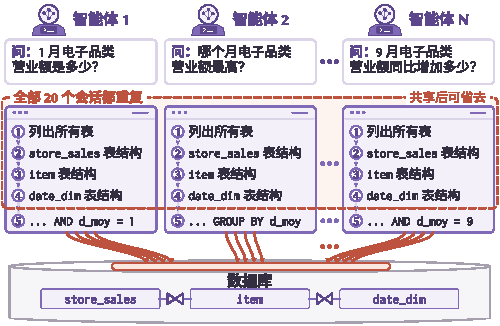
\includegraphics[width=\columnwidth]{figures/metric-record-zh}%
\else
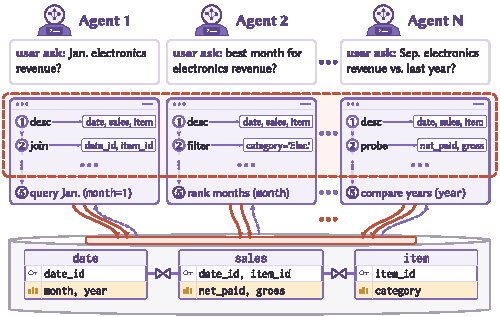
\includegraphics[width=\columnwidth]{figures/metric-record}%
\fi
\caption{\bt{Three agents asking about electronics revenue on the same database. Every session repeats steps 1--4; only the date filter in step~5 differs.}{同一数据库上询问电子品类营业额的三个智能体。每个会话都重复第 1--4 步，只有第 5 步的日期条件不同。}}
\label{fig:metric-record}
\Description{Three agent boxes, Agent 1, Agent 2 and Agent N, each show a question after the word ask: electronics revenue in January; which month had the highest electronics revenue; September electronics revenue versus a year earlier. An ellipsis between Agent 2 and Agent N marks more agents. Below them, one dashed box labelled repeated in all \WxSessions\ sessions and avoidable with sharing holds the same four steps for every agent: 1 list tables, 2 store\_sales schema, 3 item schema, 4 date\_dim schema. Under the box, each agent's step 5, final SQL, shows only its date filter: AND d\_moy = 1; GROUP BY d\_moy ORDER BY revenue DESC; AND d\_moy = 9 with GROUP BY d\_year, d\_moy.}
\end{figure}
